\documentclass{article}


\usepackage{PRIMEarxiv}

\usepackage[utf8]{inputenc} % allow utf-8 input
\usepackage[T1]{fontenc}    % use 8-bit T1 fonts
\usepackage{hyperref}       % hyperlinks
\usepackage{url}            % simple URL typesetting
\usepackage{booktabs}       % professional-quality tables
\usepackage{amsfonts}       % blackboard math symbols
\usepackage{nicefrac}       % compact symbols for 1/2, etc.
\usepackage{microtype}      % microtypography
\usepackage{lipsum}
\usepackage{fancyhdr}       % header
\usepackage{graphicx}       % graphics
\graphicspath{{media/}}     % organize your images and other figures under media/ folder

%Header
\pagestyle{fancy}
\thispagestyle{empty}
\rhead{ \textit{ }} 

% Update your Headers here
\fancyhead[LO]{NP4G : Network Programming for Generalization}
% \fancyhead[RE]{Firstauthor and Secondauthor} % Firstauthor et al. if more than 2 - must use \documentclass[twoside]{article}



  
%% Title
\title{NP4G : Network Programming for Generalization
%%%% Cite as
%%%% Update your official citation here when published 
%\thanks{\textit{\underline{Citation}}: 
%\textbf{Authors. Title. Pages.... DOI:000000/11111.}} 
}

\author{
  Shoichiro Hara \\
  Nagoya City University \\
  \texttt{s.hara@nsc.nagoya-cu.ac.jp} \\
  %% examples of more authors
   \And
  Yuji Watanabe \\
  Nagoya City University \\
  \texttt{yuji@nsc.nagoya-cu.ac.jp} \\
  %% \AND
  %% Coauthor \\
  %% Affiliation \\
  %% Address \\
  %% \texttt{email} \\
  %% \And
  %% Coauthor \\
  %% Affiliation \\
  %% Address \\
  %% \texttt{email} \\
  %% \And
  %% Coauthor \\
  %% Affiliation \\
  %% Address \\
  %% \texttt{email} \\
}


\begin{document}
\maketitle


\begin{abstract}
 Automatic programming has been actively studied for a long time by various approaches including genetic programming. In recent years, automatic programming using neural networks such as GPT-3 has been actively studied and is attracting a lot of attention. However, these methods are illogical inference based on experience by enormous learning, and their thinking process is unclear. Even using the method by logical inference with a clear thinking process, the system that automatically generates any programs has not yet been realized. Especially, inductive inference, which is logical inference to generalize from each instance, is an important issue because it can make artificial intelligence acquire knowledge by itself.
 In this study, we propose NP4G: Network Programming for Generalization, which can automatically generate programs by inductive inference. Because this is a method that can realize "sequence", "selection", and "iteration" in programming, it is satisfy the conditions of the structured program theorem. So we expect that NP4G is a method automatically acquire any programs by inductive inference.
 As an example, we automatically construct a bitwise NOT operator's program from several teacher data by generalization using NP4G. It is just randomly selecting nodes and connecting them, but by adjusting the number of nodes and the number of phase of Phased Learning, we show a bitwise NOT operator's program is acquired in a comparatively short time and at a rate of about 7 in 10 running.
 The source code of NP4G is available on GitHub as a public repository\footnotemark[1].
\end{abstract}


% keywords can be removed
\keywords{inductive inference \and automatic programming \and knowledge acquisition \and Genetic Programming \and Genetic Network Programming}

\footnotetext[1]{https://github.com/Amplil/np4g}
\section{Introduction}
Automatic programming has been actively studied for a long time by various approaches including genetic programming.
In recent years, automatic programming using neural networks such as GPT-3\cite{gpt3} has been actively studied and is attracting a lot of attention.
However, these methods are illogical inference based on experience by enormous learning, and their thinking process is unclear.
Even using the method by logical inference with a clear thinking process, the system that automatically generates any programs has not yet been realized. 
Because need to extract the structure of some kind of solutions to the problem comes out to realize automatic programming by this logical reasoning, it is the related field that is deep with the acquirement of knowledge of the artificial intelligence.
In the study on acquirement of knowledge of the artificial intelligence, there is still that what's called knowledge includes a lot contradiction or an exception and is hard to formulate it as a big problem.
The inductive reasoning generalized by logical reasoning from one example can acquire artificial intelligence oneself knowledge and is an important problem particularly each.
In this study, we propose NP4G: Network Programming for Generalization, which can automatically generate programs by inductive inference.
Because this is a method that can realize "sequence", "selection", and "iteration" in programming, it is satisfy the conditions of the structured program theorem. So we expect that NP4G is a method automatically acquire any programs by inductive inference.
As an example, we automatically construct a bitwise NOT operator's program from several teacher data by generalization using NP4G.
It is just randomly selecting nodes and connecting them, but by adjusting the number of nodes and the number of phase of Phased Learning, we show a bitwise NOT operator's program is acquired in a comparatively short time and at a rate of about 7 in 10 running.
I show automatic programming, inductive reasoning, genetic programming as a related study in two chapters as follows.
I suggest network programming (NP4G) for generalization in three chapters and explain the fabric.
I speak a method getting the bit NOT operation program for one of the suggestion technique in four chapters and I show the inspection result in five chapters and examine it.
I show the significance of this study and a future problem in six chapters.
The source code of NP4G is available on GitHub as a public repository \footnotemark[1]. 


\section{Related Research}
\subsection{Automatic Programming}
\label{sec:headings}
Automatic programming (AP:Automatic programming) is that all to a part automate the generation of the program and puts the success that is constant as assistance of the developer in from a large-scale system to a small program \cite{AutomaticProgramming}. 
In automatic programming, as for the model to generate a program automatically, a study is done for a long time by logical reasoning.
Logic Theorist which was the world's first artificial intelligence program announced in 1956 intended to imitate human logical reasoning using a search tree and Hugh squirrel Thich, and was made \cite{LogicTheorist}.
In late years there is the technique using the large-scale language model by the neural network represented as a study of the automatic programming attracting attention by GPT3\cite{gpt3} of OpenAI.
By, from the enormous cords which are opened to the public, learning it as a language model by the depths learning, predict a cord depending on the situation, and this is the technique that it is automatic and generates.
Where these technique predicts the code that the developer is going to write on an editor, and the continuance is applied to a function suggesting and puts big success in \cite{copilot}.
However, We do not generate a code by logical reasoning because these technique is language generation models and are the reasoning based on the illogical experience by enormous learning.
In this respect, it may be said that many tasks are left in the present age.
In addition, by generation of the automatic programming by the logical reasoning, I gain constant result even recently, but a problem remains only for a language peculiar to domains such as \cite{palsql}, the SQL at a point called the acquisition of the option program because it is effective technique.

\subsection {Inductive Inference}
In a wide sense, logical inference consists of deduction reasoning, inductive inference and analogical inference \cite{math300}.
As a representative thing of the logical thought, "an inductive way of thinking", is \cite{saito:11}. with "a way of thinking of the encoding" "a way of thinking of the generalization" "an analogy-like way of thinking"
Of these, it is "a way of thinking of the generalization" to be equivalent to inductive reasoning.
Inductive inference is the reasoning to arrive at a general rule to explain that from given data \cite {inductive-reasoning}.
The inductive reasoning with the artificial intelligence is studied for a long time, but \cite{CASE1983193}\cite{4767034}, coverage are restrictive, and a task is left in any program.
In addition, connection is deep with the study of the acquirement of knowledge because the inductive reasoning with the artificial intelligence can say that it is a method to acquire knowledge automatically.
There are the things which contradict it between rules even if I formulated a lot of things which I cannot formulate in the knowledge and I say such a problem with an acquirement of knowledge problem and am not still solved \cite{KnowledgeAI}\cite{KAIssues}.
As the technique of the neural network can pick out the common point of the characteristic of individual data if I say at a point of view called the generalized reasoning, it may be said that it is the range of this field.
However, it is not logical because I sought a correlation based on enormous data.
In addition, \cite{BlackBoxProblem}. where the judgment process lacks in explanation characteristics, and this problem is called the issue of flight recorder
In addition, a large quantity of data are necessary for learning and are the reasoning that is generalized from this, but it is revealed that it is not inductive reasoning.
\subsection {Genetic Programming}
Genetic programming (GP) is technique by to use genetic operation, generate a program of the hierarchy structure automatically \cite{Koza1994}.
It is used for the solution to various problems including several sets of automatic construction and generation of the action subsidiary of agent.
GNP (Genetic Network Programming) deals only with hierarchy structure by the GP, but the thing which expanded this in the network is hereditary network programming \cite{gnp}.
By turning the smallest unit and a thought, those way of combining taking a simple step automatically, with GP/GNP, the most suitable program builds each node of the network.
I can classify each node in a judgment node, a processing node, a start node mainly.
With GP/GNP, I can get an expressed program automatically by a network, but I cannot see the example which applied to inductive reasoning.
\section {Proposed Method}
\subsection{Basic Concept of NP4G}
NP4G is technique by to generate a program expressed in a network automatically, perform inductive reasoning based on teacher data.
For example, in \ref{fig:summary}, I get a bit NOT operation program by generalization from four teacher data.
Teacher data are data of 1 input 1 output and search until the program that input and output in accordance with the teacher data is provided is generated.
The generated program is provided as well as a way of thinking of the GNP by connecting the plural nodes with the simple function into a network form.
The GNP is network programming using the hereditary technique, but NP4G is technique assuming an application of various technique not only use of the hereditary technique.
By being generalized for one example (teacher data) each, in NP4G, it may be said that it is technique of the acquirement of knowledge by the inductive reasoning in the point to acquire one knowledge (program).
Therefore there is very few it and, unlike the technique using the neural network, finishes the number of necessary teacher data with around several which can get a target characteristic to be generalized.
In addition, it is apparent as built program itself becomes the form of the network whether you work what kind of inside.
The attempt to automatically generate a program by the combination of networks has been used only in hereditary technique of the GNP conventionally.
However, I use network programming as means to be generalized by the suggestion technique.
When the network programming not to be limited to this hereditary technique is applied as new automatic programming technique widely in the new field in future, I can hope.
As well as GP/GNP, I can expect expansion to the effective algorithm by the combination with other technique of neural network or reinforcement learning in future.
\begin{figure}[t]
\begin{center}

\includegraphics[width=80mm]{summary.png}
\end{center}
%\capwidth=80mm %
\caption {Generalization from teacher data}
\label{fig:summary}
\end{figure}
\subsection {Structured Theorem}
A use had a problem that it was restrictive with the technique that logical reasoning had.
However, it has structure to meet the condition of the structured theorem to obtain any program in NP4G.
With the structured theorem, any program is three kinds of \cite{StructuredProgramming}. which is a fabric, a theorem to insist that I can constitute it by a combination "repeatedly" "a choice" "sequentially"
Because NP4G can realize "a choice" by the data which are iterable "repeatedly" to explain it in \ref{sec:struct} by establishing a judgment node and the processing node for a function to be given beforehand "sequentially" by carrying out a node by the order that I was able to decide from a start node, it may be said that I meet the condition of the structured theorem.
\subsection{Basic Structure of NP4G}
\label{sec:struct}
NP4G has the effective graph structure that the node such as plural functions and objects was connected to into a network form like \ref{fig:sequence}.
As for the node, there are not a function (squares in a figure), a start node (circle written as "S" in a figure) having the input data carried out first of the program, an end node (circle written as "E" in a figure) informing the end of the program, a link of the input and is classified roughly in an object node (circles in a figure) to output data stored beforehand.
The number of links connected as input of the node varies according to functions, but the number of it is how many and can connect the number of the link of the output without depending on a function.
\subsubsection {Execution Order of Nodes}
\label{sec:sequence}
Using an example of the network produced in NP4G which I showed in \ref{fig:sequence}, I explain the order of practice of the node.
As a node is handled sequentially by a start node, of the structured theorem can come true "sequentially".
At first, a node connected to a start node having input data is carried out with \textcircled{\scriptsize 1}, \textcircled{\scriptsize 2}, \textcircled{\scriptsize 3} sequentially by the top.
If all those nodes are carried out, the node connected to those nodes is carried out with \textcircled{\scriptsize 4}, \textcircled{\scriptsize 5}, \textcircled{\scriptsize 6} sequentially equally by the top.
When I catch a network as data subsidiary, I set a node carried out next as a list, and the operation to carry out sequentially from this top means operation to carry out sequentially for some time.
When there is not the output from other nodes to become the input yet, it is in "not yet", and, here, the practice result is not output like \textcircled{\scriptsize 4} of \ref{fig:sequence}.
When there is a node not to be derived from a start node like \textcircled{\scriptsize 9}, this means that it is not output.
On the other hand, it is output because \textcircled{\scriptsize 5} is carried out in the case of \textcircled{\scriptsize 6} just before that, and all the output of the node to become the input exists.
It is carried out with \textcircled{\scriptsize 7}, \textcircled{\scriptsize 8}, \textcircled{\scriptsize 9} next, but the practice result becomes "already done" as this node has been already output in \textcircled{\scriptsize 6} in the case of \textcircled{\scriptsize 8}, and there is not the thing output again.
In this way, each node is carried out until a node handled next disappears.
An output node takes the output of the whole network last and is finally connected to the end node.
In other words, the end node is not connected to the network from the cost and can decide it from relations of the order of practice of the node subsequently.
\begin{figure*}[t]
\begin{center}
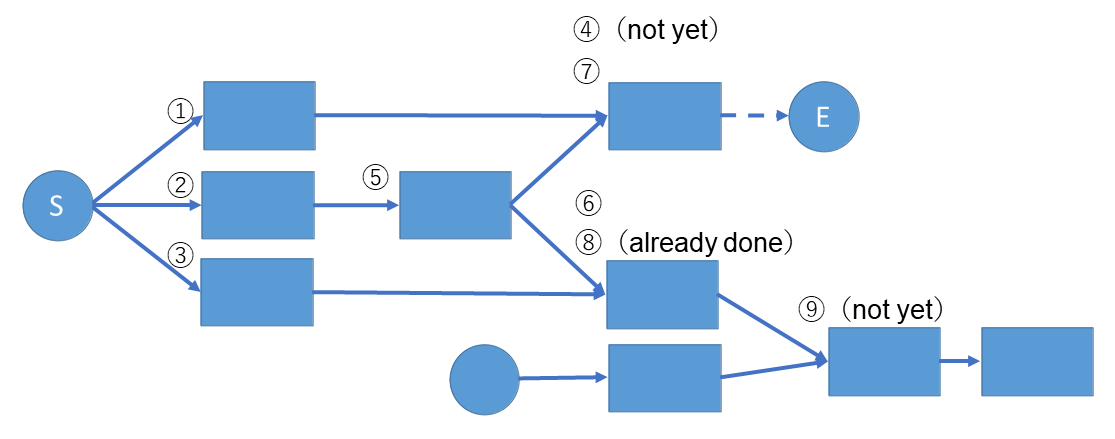
\includegraphics[width=130mm]{sequence.png}
\end{center}
%\capwidth=90mm %
A fabric and order of practice of \caption{NP4G}
\label{fig:sequence}
\end{figure*}
\subsubsection {Iteration}
It is necessary to introduce "iteration" to meet a structured theorem.
I realize it by letting a function input the data which are iterable not realizing iteration by making feedback loop on the network in NP4G.
The function that the data which are iterable were given as input carries out the same processing for each element of the data.
A function performs the handling of data to return to the data which are not generation or iterable which are iterable, and I repeat it as far as the data which are iterable are used as input of the function, and processing is done.
I can realize iteration without a program without by doing it this way, falling into an infinite loop, and being finished being made.
In addition, it becomes hard to cause an error when I put a node together at random and generate a program automatically as much as the order of practice of the node becomes concise.
\subsubsection {Automatic Definition Functions (ADFs)}
By the GP, a definition function (ADFs: Automatically Defined Functions) automatic in the case of the evolution of the program speedup expecting it is used \cite{adfs}.
ADFs makes possible by to reuse the network which was already completed, make a higher program within a short time.
I register a network as ADFs every stage and, in NP4G, allow you to reuse the network at the next stage in combination with phased learning to explain ADFs in \ref{sec:PL}.
\subsubsection {Phased Learning}
\label{sec:PL}
It is technique to let you learn it without unreasonableness even if it is a complicated program by the phased learning (Phased Learning) distributing learning for each stage, and performing it.
\cite{hodohara2012reinforcement}. where an effect by that the phased learning is technique used in reinforcement learning mainly and lowers the flexibility that I can take of the learning, prevents that learning time becomes enormous is seen in
In NP4G, I reduce the number of teacher data letting, at first, you learn it, and a network taking a simple step starts with being produced.
And I reuse a produced network when I build a network next as ADFs.
I can hope that I learn it in a shorter time than time by to do it this way, get a complicated network from the beginning.
\section {Acquisition of a Bitwise NOT Operator's Program}
I think about a case to automatically build a bitwise NOT operator's program to be concrete and, using NP4G, inspect it by actually executing a program of NP4G.
I program NP4G using Python(Python 3.7.12) that is a programming language in this study.
As practice environment, I use Colaboratory of Google.
In addition, as the data which are iterable to realize iteration, I use a list-shaped object (the following, list) on Python program.
In NP4G, all the data stored away in teacher data and a start node, an object node are character string.
\subsection {Preliminarily Provided Functions}
The node to be given for functions to build a network beforehand assumes it four of split function, sum function, an equal function, the control gate function to show it in \ref{fig:func}.
I explain the contents of each function as follows.
\subsubsection{Split Function}
As an end, I distribute character string and make space list notation.
When I show it in a figure, I keep you and transcribe "split" in a square.
\subsubsection{Sum Function}
I smooth it for list-shaped input and plural input including other character string and do it for one character string by catching it between character string in space, and being connected.
Character string of the input is "[NULL]
When is ", "[NULL]
"Is not connected.
When character string of the output is "" (the sky), "[NULL]
It outputs ".
When I show it in a figure, I keep you and transcribe "+" in a square.
\subsubsection {Equal Function}
Time "[TRUE] where a value of two input accords
It outputs ".
Other than that, it is "[FALSE]
It outputs ".
I play a role as the judgment node in GP/GNP.
When I show it in a figure, I keep you and transcribe "= =" in a square.
\subsubsection {Control Gate Function}
Among two input, either is "[TRUE]
When is ", other than that, through a value of the other input, is "[NULL]
It outputs ".
I play a role as the processing node in GP/GNP.
When I show it in a figure, I write it in Shiromaru.
\begin{figure*}[t]
\begin{center}
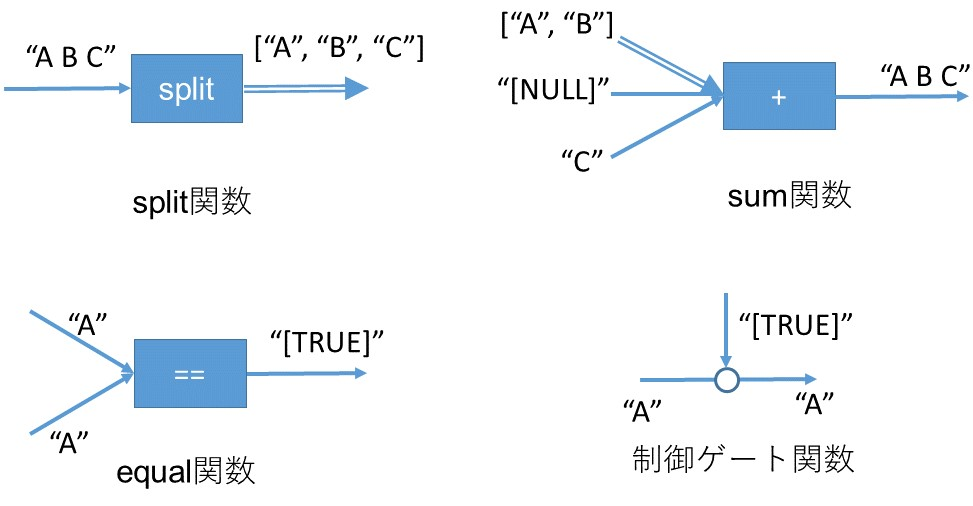
\includegraphics[width=110mm]{func.PNG}
\end{center}
%\capwidth=90mm %
\caption {Function to be given beforehand}
\label{fig:func}
\end{figure*}
\subsection {Example of a Bitwise NOT Operator's Program}
I show the example of the bit NOT operation program that is realized by using these four functions in \ref{fig:bitwise_not}.
At first, I build the left upper network of the figure for input of 1 bit as the first stage.
An equal function to have the start node that stored away object node and input "0" which stored away "0" for input is "[TRUE]
It outputs ".
"[TRUE]
A control gate function to have "toward input just outputs the value of the object node that stored away" 1 ".
I realize "the choice" of the structured theorem by an equal function and a control gate function in this way.
And it is "[FALSE] for input "0"
"And "[NULL]
Another equal function and control gate function to output ", in the case of" 1 ", input is "[TRUE] each
I build logic not of 1 bit as a network by outputting "and" 0 ".
\begin{figure*}[t]
\begin{center}
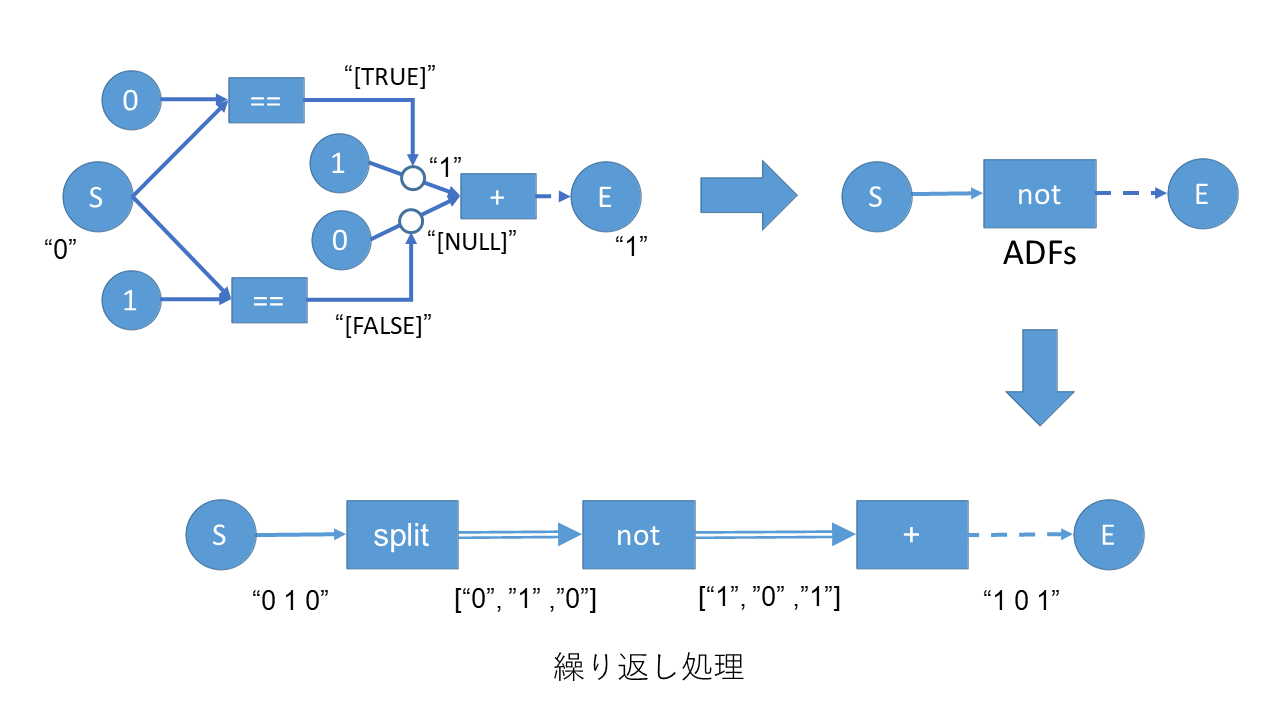
\includegraphics[width=150mm]{bitwise_not.png}
\end{center}
%\capwidth=130mm %
Implementation of a bit NOT operation program by \caption{NP4G}
\label{fig:bitwise_not}
\end{figure*}
Then, I do it in the form that the construction of the next network can reuse this network as ADFs to show it in the top right corner of the figure.
In the figure, I keep you and transcribe "not" in a square.
And I build a bit NOT operation program by using repeated handling of data (list) which are iterable and "not" of ADFs during the next stage to assume plural bits input.
I make the input character string of plural bits a list by split function and I repeat "not" which is ADFs for individual elements and apply it and connect scattered character string by sum function and realize logic not of the plural number bit.
By performing phased learning to step on a stage in this way, and to build a network, realize an objective program.
\subsection {Inspection Method}
I choose the node at random and, for several teacher data, just tie it and inspect whether it is automatic, and you can acquire a bit NOT operation program by NP4G.
\subsubsection {Teacher Data and Random Search}
The teacher data to use are four to show in \ref{tbl:TeacherData}, and teacher data used at each stage by a method of the phased learning change.
In addition, I write a parenthesis like (input, the output), and each input and output of teacher data writes it.
\begin{table}[htbp]
\centering
\caption {All of teacher data to use in this study}
\label{tbl:TeacherData}
\begin{tabular}{l}
\hline
(input, output) \\
\hline \hline
( "0" , "1" ) \\
( "1" , "0" ) \\
( "0 0" , "1 1" ) \\
("0 1 0" "1 0 1") \\
\hline
\end{tabular}
\end{table}
I search for the network which is equal to these teacher data of each stage as automatic generation of the bit NOT operation program by NP4G by putting a node together at random.
At first, I put an end node, and only the number of the nodes that I was able to decide chooses a node with a start node at random, and the random algorithm ties only the number of of the input of the function with other nodes at random next.
\subsubsection {Method of the Phased Learning}
\label{sec:PLhow}
Here, I prepare for a stage to use it by phased learning until 5 for a stage from 1 for a stage and by changing the pair of each stage, check influence of the phased learning.
Five teacher data at the stage to use by phased learning are as follows.
\begin{itemize}
\item Phase 1: ("0", "1")
\item Phase 2: ("1", "0")
\item Phase 3: ("0", "1"), ("1", "0")
\item Phase 4: ("1", "0"), ("0 0", "1 1")
\item Phase 5: ("1", "0"), ("0 0", "1 1") ("0 1 0", "1 0 1")
\end{itemize}
And 3 each phases
\begin{itemize}
\item 3 phases:
Phase 2, 3, 4
\item 4 phases:
Phase 1, 2, 3, 4
\item 5 phases:
Phase 1, 2, 3, 4, 5
\end{itemize}
\noindent
I change the number of the stage and compare this.
By adding it to a list using lambda expression of Python as ADFs, can reuse the network provided at each stage at the next stage and do it.
I search for the network which is equal to the teacher data of each stage by putting function and object node, ADFs given beforehand together at random.
In addition, it is necessary for the object node to prepare like a function to be given beforehand beforehand.
In the case of an object node, I prepare input of teacher data to use by the learning of each stage and both character string of the output as an object node.
\subsubsection {Inspection}
By the inspection, I carry out ten times of programs of NP4G and seek the generation result and the mean of the execute time.
When it is not generated "failure" before a time limit in the practice of one program when "success" is not so if the network which the generation result searches, and was provided is a generalized network to be able to get the output to expect from, I say with "excess".
I check whether it is the output to expect by inputting all binary character string (from "0" "1 1 1 1 1") from one digit to five digits as inspection data.
In addition, I do it with three hours (10,800 seconds) in a time limit in one practice.
\section {Results and Considerations}
I show the practice result of the program of NP4G when I changed a number and the number of the nodes of the stage in \ref{tbl:result1}.
I arrange each number of "the excess", and, as for the practice result, "failure" shows "success".
In addition, I show average, maximum, a minimum of each execute time (s) when I changed a number and the number of the nodes of the stage in \ref{tbl:result2}.
The number that four phases, time of 20 number of the nodes succeeded in from \ref{tbl:result1}, \ref{tbl:result2} is relatively short with 1,105s in seven and most, average time.
In addition, at the time of four phases, number of the nodes 15, the number of the success is six, but, as for the average time, is the shortest with 334s.
It may be said that these are the best results.
Four phases of networks where I failed in were only one case at the age of ten number of the nodes to know it from \ref{tbl:result1}.
In addition, it was all excess only except one case of the success at the age of five phases at time when I saw a result at the age of the number of the nodes 5.
It is thought that this is because there were too few nodes that this is the number of five nodes and generates a bit NOT operation program.
On the other hand, in the numbers that the number of the nodes becomes the excess like 20 at time when with much number of the nodes tending to increase, it is thought that this is because time suffers from the generation of the network as much as the number of the nodes increases.
Then, it turns out that I tend to have a long three phases of average time when I see the average time every number of the stage in \ref{tbl:result2}.
As this has few numbers to go through a stage with three phases, it is thought that this is because need to make the complicated network with once comes out.
In addition, as for the reason why five phases tend to have a long average time than four phases, it is thought that this is because it takes time extra by just that much if I increase too many stages.
I show a network of the number of five phases of successful nodes 5 in \ref{fig:out_net_p5n5} by automatic generation with the number of the nodes 5 alone.
When there was little number of the nodes, like this network, it turned out that I could get a network to expect.
After having generated a network becoming 1 output for 0 input in 1 for a stage automatically, it is used as adf1 in 2 for a stage, and, in the network made with 2 for a stage, it is revealed that it is used as adf2 by 3 for a stage.
It is revealed that there is already the network which I nominated for an implementation of the bit NOT operation in \ref{fig:bitwise_not} by 4 using adf3 for a stage.
A bit NOT operation program was provided at 4 for a stage, and, in the case of this network, it was revealed that a network but to expect was provided in the middle of phased learning.
Then, I show a network when I failed by automatic generation with the number of four phases of nodes 10 in \ref{fig:out_net_p4n10}.
In this way, it is thought that the output becoming mismatched by the inspection data has come out to the output which fits all it for the teacher data although I appear because it has become the complicated network.
In the case of this network, it became "0 1 1" for input of "0 1 0" and became the output which was not "1 0 1".
Even in this case I increase stages, and it is thought that a network by to learn ("0 1 0", "1 0 1") by the teacher data which I included, expect is provided.
In addition, it is necessarily revealed that I may not use adf1 and adf3 which are generated ADFs by a previous stage from 4 for 2 and a stage for a stage of \ref{fig:out_net_p4n10} to choose a node at random when I build a network.
As can be seen, in NP4G, a thought process is clear unlike the technique using the neural network in a network provided by \ref{fig:out_net_p5n5}, real inspection of \ref{fig:out_net_p4n10}.
I show average, maximum, a minimum of (s) in \ref{tbl:result3} at the generation time in each stage.
This table added it up from all successful results regardless of the number of the nodes and the number of the stage.
From this table, it turns out that it has a shorter generation time in 1,2 than other stages for a stage.
Even if stage 1, 2 is the generation of the random network because teacher data are learning only for one set together, in this, it is thought that this is because a network in accordance with teacher data is easy to be found.
Then, average of the generation time in 3 gets longer most with 2585.24s for a stage, and 4 understands that 5 is long next next for a stage for a stage.
I think about these factors.
At first, it is thought that this is because it was necessary to generate a complicated network because it is teacher data ("0" "1"), ("1", "0") learning, and it is necessary to search for a network meeting two conditions for the first time in one network in the case of 3 for a stage.
In the case of 4, the complicated network is not required for a stage, but it is thought that generation time got longer as it was necessary to generate the network which is repeated for the first time in 4 for a stage, and needs processing.
It is thought that I was able to control generation time briefly because I can cope in the same network even if figures increased after having learned iteration in the case of 5 for a stage.
\begin{table}[htbp]
\caption {Practice result (success/failure/excess)}
\label{tbl:result1}
\begin{tabular}{c|cccc}
Number of the nodes &
5&
10&
15&
20\\
\hline \hline
Three phases of &
0 / 0 / 10&
8 / 0 / 2&
6 / 0 / 4&
2 / 0 / 8\\
Four phases of &
0 / 0 / 10&
7 / 1 / 2&
6 / 0 / 4&
7 / 0 / 3\\
Five phases of &
1 / 0 / 9&
6 / 0 / 4&
7 / 0 / 3&
5 / 0 / 5\\
\hline
\end{tabular}
\end{table}
\begin{table}[htbp]
\caption {Execute time (s)}
\label{tbl:result2}
\begin{tabular}{c|crrrrr}
Number of the nodes & & 5&
10& 15&
20\\
\hline \hline
&
Mean & -& 3067& 5565& 3699\\
Three phases of &'s greatest & -& 10480& 8966& 9543\\
&
Smallest & -& 258&
1&
3\\
\hline
&
Mean & -& 3024& 334& 1105\\
Four phases of &'s greatest & -& 8294& 1103& 2835\\
&
Smallest & -& 134&
7&
10\\
\hline
&
Mean & 32& 4090& 1506& 1266\\
Five phases of &'s greatest & 32& 9103& 7866& 2586\\
&
Smallest & 32&
1&
2& 26\\
\hline
\end{tabular}
\end{table}
\begin{table}[htbp]
\caption {Generation time (s) in each stage}
\label{tbl:result3}
\begin{tabular}{c|rrrrr}
Stage &
1&
2&
3&
4&
5\\
\hline
\hline
Mean &
1.17&
2.24&
2585.24&
188.31&
12.49\\
Maximum &
6.94&
24.20&
10425.58&
1114.09&
347.02\\
Smallest &
0.00&
0.00&
0.53&
3.95&
0.03\\
\hline
\end{tabular}
\end{table}
\begin{figure*}[t]
\begin{center}
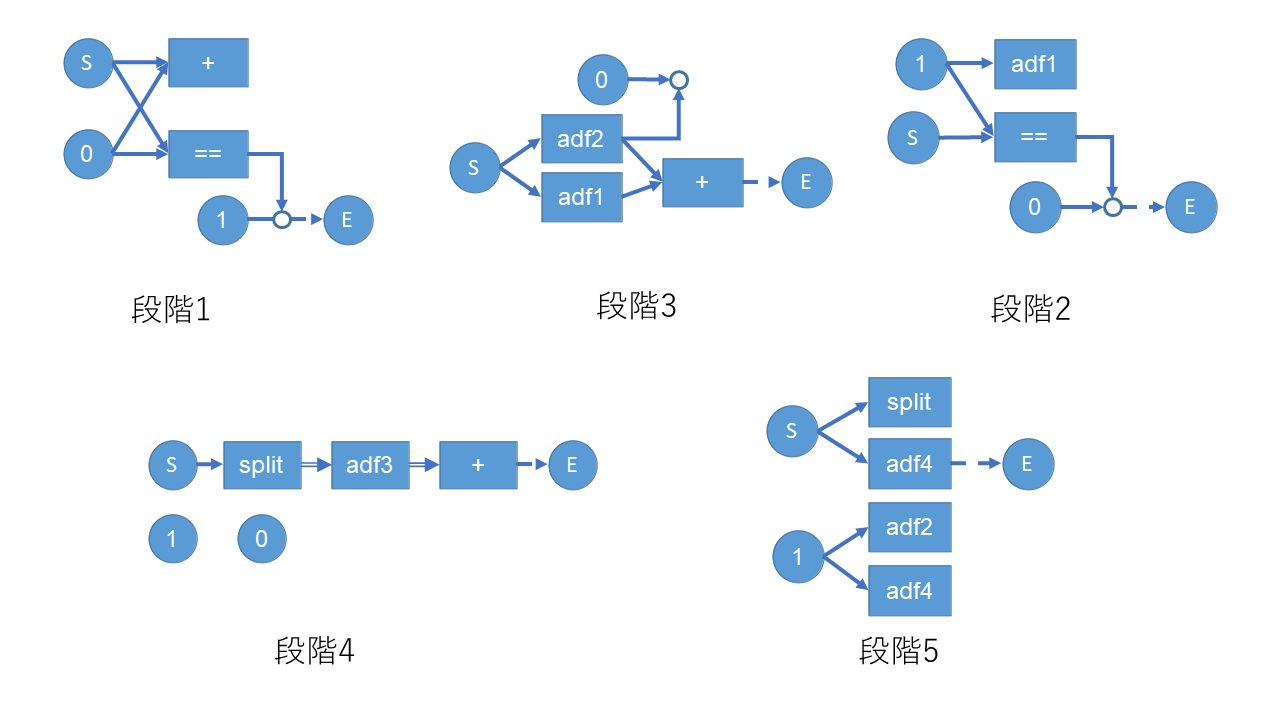
\includegraphics[width=150mm]{out_net_p5n5.png}
\end{center}
%\capwidth=130mm %
\caption {Network when a program to expect by automatic generation with the number of five phases of nodes 5 was provided}
\label{fig:out_net_p5n5}
\end{figure*}
\begin{figure*}[t]
\begin{center}
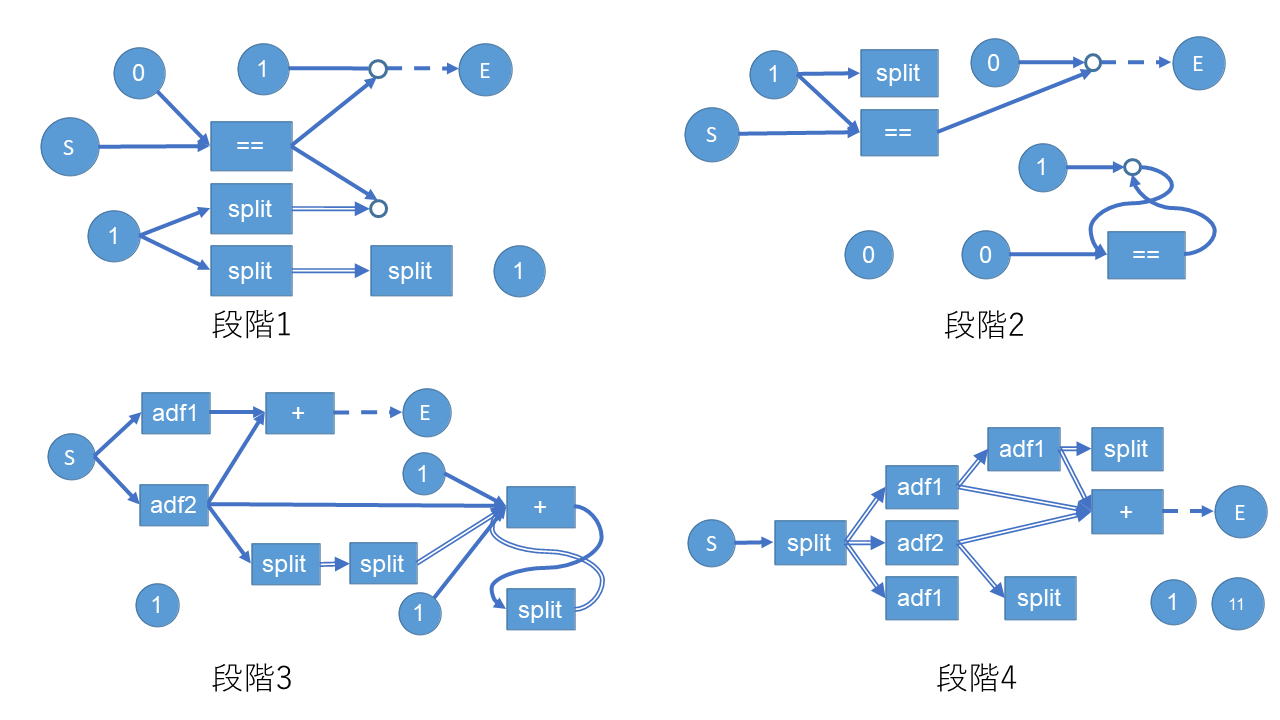
\includegraphics[width=150mm]{out_net_p4n10.png}
\end{center}
%\capwidth=130mm %
\caption {Network when the input and output accorded with the teacher data which I used for learning by automatic generation with the number of four phases of nodes 10, but the program that was different from expectation was provided}
\label{fig:out_net_p4n10}
\end{figure*}
\section {Conclusion}
\subsection {Summary and Significance in this study}
In this study, I suggested network programming (NP4G) for generalization.
By using NP4G, chose the node at random and just tied it, but confirmed that I could acquire a bit NOT operation program from several teacher data.
As NP4G is technique finding a general property from several examples, it is inductive reasoning.
In addition, it has the structure that "a choice" meets the condition of the structured theorem "repeatedly" "sequentially" in the programming and is the technique that it can expect to acquire any program by inductive reasoning automatically.
When the network programming not to be limited to hereditary technique shown by NP4G is applied as technique of the new automatic programming widely in the new field in future, I can hope.
There is it at the point that showed that I can expect realization of the artificial intelligence which general-purpose, is flexible which learns the significance of this study for every knowledge by network programming by oneself, and makes use of the contents, and reasons for a different problem logically, and leads an answer.
\subsection {Issues}
\subsubsection {Turing Completeness}
Indicating NP4G having explained that meet the condition of the structured theorem, but NP4G being Turing perfection to prove that NP4G is technique to be provided by any program it is necessary.
If Turing is complete, a certain calculation model has the computing power that is equal to all-around Turing machine, in other words, show what can reproduce any program.
I mean that the technique that can get any program by inductive reasoning was able to be realized if I can show that Turing is complete.
In addition, it is necessary to actually try whether you can automatically build not only the bit NOT operator but also other programs using NP4G.
\subsubsection {Grouping for a Search Technique}
In this study, I used an accidental search by the random generation as search technique of the network.
A type and the number of nodes to use increase because this technique is a primitive, and time suffers from a search so that an objective program is complicated.
I use reinforcement learning and by combining it with other learning technique, it is automatic and adjusts a type and a number, the way of the node deserving to be a component of the network of combining, and it will be necessary to plan efficiency of the network construction in future.
\subsubsection {Evaluation of the Network}
By hereditary technique and other learning technique including the reinforcement learning, it is provided with the mechanism that a number evaluates a generated network and model using evaluation function.
In this study, it becomes the evaluation whether or not an objective network was produced, and there is not a number evaluation by the evaluation function.
I can change the architectural way by the evaluation of the network in future if I can establish the evaluation method of the network in NP4G.
In addition, it becomes easy to combine it with other learning technique using the evaluation function.
\subsubsection {Simplification of the Network}
Even if a node was in the network in NP4G as explained in \ref{sec:sequence}, the node is not carried out when it is not a node to be derived from a start node.
When such a node comes out, if there are any the algorithm that I remove after having produced a network, I can plan the simplification of the produced network.
\section*{Acknowledgments}
This study is supported by JPMJSP2130: Pioneering Research Initiated by the Next Generation in the JST.


%Bibliography
\bibliographystyle{unsrt}  
\bibliography{btx_np4g}  


\end{document}
